\documentclass[11pt,a4paper]{article}
\usepackage[utf8]{inputenc}
\usepackage[spanish]{babel}
\usepackage[pdftex]{graphicx}
\usepackage{color}
\usepackage{pdfpages}
\usepackage{url}

\title{Práctica Nagios}
\author{Nombre del estudiante que realiza el trabajo}
\date{Diciembre 2014}

\begin{document}

\maketitle
\tableofcontents
\clearpage

\section{Introducción a Nagios}

Aquí se debe introducir la definión de qué es Nagios\cite{web}. Sería deseable que introdujérais también 
otros sistemas similares a Nagios.

\section{Funcionamiento de Nagios}

Explicación de cómo funciona Nagios

Se pueden incluir figuras como por ejemplo la Figura~\ref{figura1} de la página \pageref{figura1}

\begin{figure}
\centerline{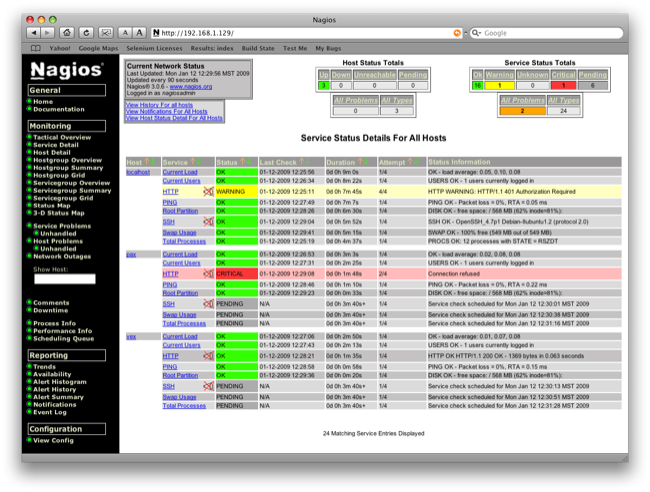
\includegraphics[width=6cm]{nagios3-1.png}}
\caption{Figura de ejemplo}
\label{figura1}
\end{figure}

\section{Instalación de Nagios}

Se explica cómo instalar Nagios. Sería conveniente que supiéseis instalar Nagios tanto utilizando
la distribución de paquetes del sistema operativo como a partir de los códigos fuente.

\section{Acceso a Nagios mediante el navegador}

Se debe explicar cómo se debe configurar el servidor web para acceder a Nagios a través del navegador
y  tambíen la interfaz web que presenta Nagios.

\section{Configurar Nagios}

Se debe explicar los distintos ficheros de configuración de Nagios y cómo se configuran para 
monitorizar tanto al sistema local como a sistemas remotos.

\section{Experiencia de instalación y configuración de  Nagios}

Se deben detallar los pasos que se han seguido para la instalación y configuración de Nagios
tanto para monitorizar el sistema local como sistemas remotos.

\begin{thebibliography}{1}

\bibitem{web} Página web del proyecto de Nagios: \url{http://www.nagios.org}

\end{thebibliography}

\end{document}
